\documentclass{article}

\usepackage{amssymb}
\usepackage{braket}
\usepackage{listings}
\usepackage{graphicx}
\usepackage{amsmath}
\usepackage{url}

\title{Homefun 2}
\author{Ben Gamari}

\begin{document}
\maketitle

\newcommand{\norm}[1]{\ensuremath{\left\lVert #1 \right\rVert}}
\newcommand{\twonorm}[1]{\ensuremath{\norm{#1}_2^2}}
\newcommand{\epi}{\ensuremath{\mathrm{epi}}}

\section{Question 1}

In order for $f : X \rightarrow Y$ to be convex, we must show that its
epigraph $F = \epi f = \{ (x,y) \vert y \ge f(x)~\forall x \in X \}$
is closed (that is $\mathrm{cl} F = F$).

As all of the $f_j$ are convex, we know that $\epi f_j$ are
closed for all $j$. Under our definition of $f$, we can consider $\epi
f$ to be the intersection of all $\epi f_j$. By nearly any
introductory topology text (e.g. Mendelson's {\it Introduction to
Topology}, Dover 1990) we know that the intersection of any number of
closed sets is itself closed.

Assuming we have a subgradient $g_i(x) = \partial f_i(x)$ for each
$f_i$, we can define the subgradient $g(x) = \partial f(x)$ to be
the corresponding subgradient $g_j$ of the maximal function $f_j \ge
f_i \forall i \ne j$. At points where multiple functions are maximal,
we may choose from the subgradients of any of these maximal functions.

In the case of $f(x) = \norm{x}_1$, we note that we can express this as,
\[ f(x) = \mathrm{max} \{ x_1 x_2 \ldots x_N, (-x_1) x_2 \ldots x_N, \ldots, (-x_1) (-x_2) \ldots (-x_N) \} \]
Using the rule proposed above, we can take $g(x) = TODO$

\begin{figure}
  \center
  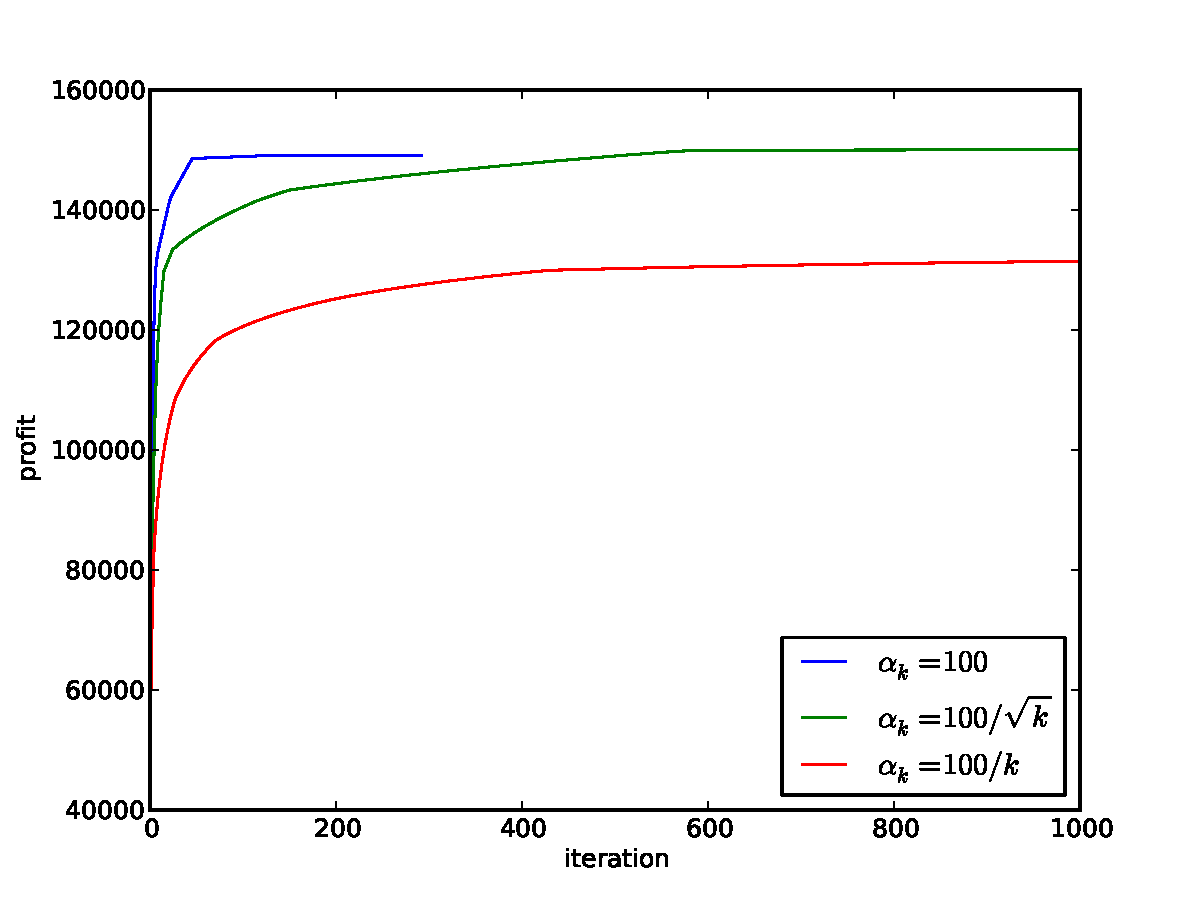
\includegraphics[scale=0.5]{q1-convergence.pdf}
  \caption{(Question 1) Convergence of projected subgradient method
while minimizing the linear program described in Question 2 of Homefun
1 for three step size schedules.}
  \label{Fig:Q1Convergence}
\end{figure}

See attached for implementation.

\section{Question 2}

We note that due to the fact that we are in a bounded space, $R =
\sqrt{2}$. As our function is strongly convex, we have that that the
Hessian is bounded such that for some $m > 0$,
\[ \nabla^2 f \ge m I \]

Consequently, the difference between the objective's optimal value
$f^*$ and the value at $x$ is bounded as a function of the gradient,
\[ f(x) - f^* \ge \frac{1}{2m} \vert \nabla f(x) \vert^2_2 \]

In general, we can still say little about the behavior of
the objective function and therefore $G$.

We recall from the lecture notes that in the case of a convex function,
\[ \twonorm{x_k - x^*} \vert_2^2 \le \twonorm{x_1 - x^*}
   - 2\alpha_k (f \]

Therefore in the case of a schedule of step sizes which is square
summable but not summable we find,
\[ f_\mathrm{best}^{(k)} - f^* \le \frac{R^2 + G^2 \twonorm{\alpha}}{2 \sum_i \alpha_i} \]

\begin{figure}
  \center
  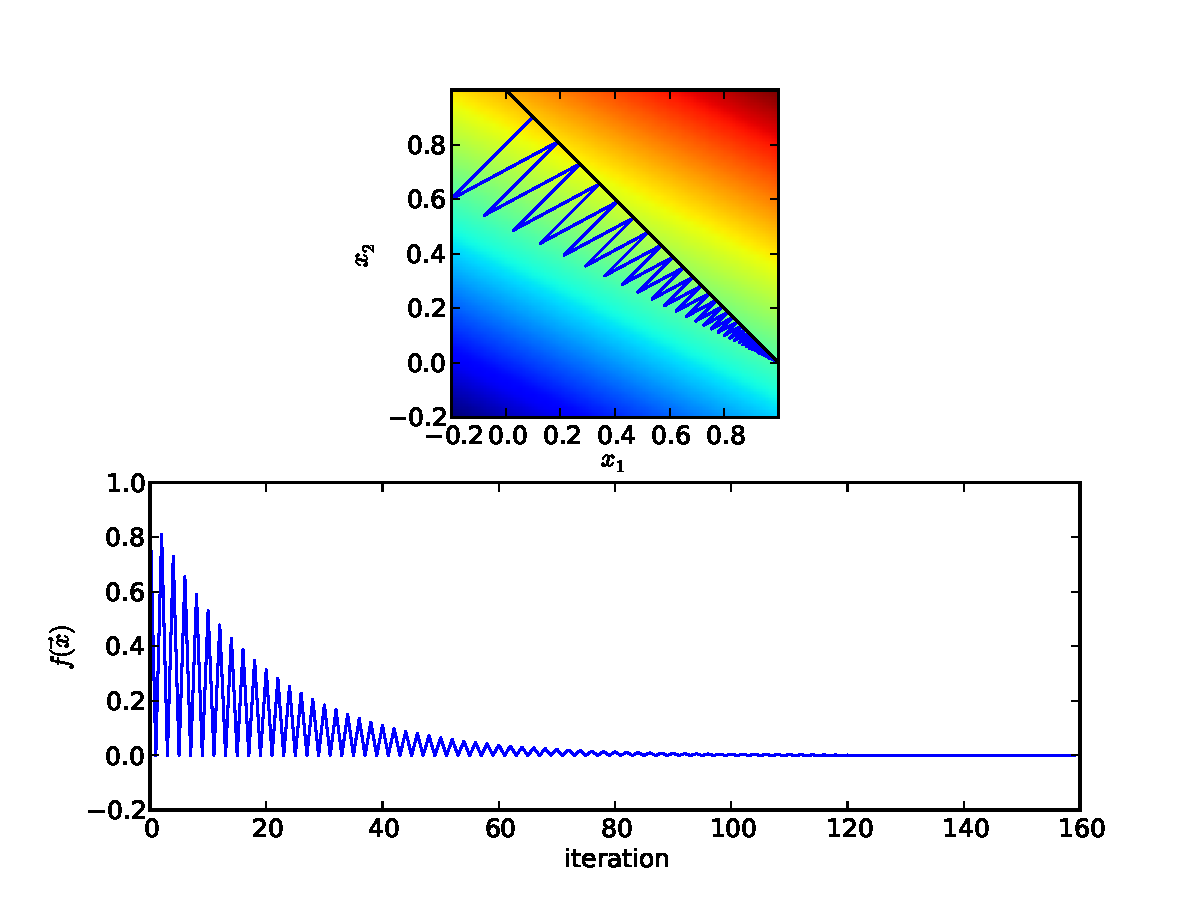
\includegraphics[scale=0.2]{q2-convergence.pdf}
  \caption{(Question 2) Convergence of projected subgradient method
while minimizing the linear program $f(x) = x_1 + 2x_2 - 1$ such that
$x_1, x_2 \ge 0$ and $x_1 + x_2 = 1$ under the step size schedule
$\alpha_k = f(x_k) / \norm{\langle 1,2\rangle}$.}
  \label{Fig:Q2Convergence}
\end{figure}

\section{Question 3}

\begin{enumerate}
\item[\bf part a]
  Recall that a function $f$ is Lipschitz smooth with constant $L_f$
  if $\twonorm{\nabla^2 f(x) - \nabla^2 f(y)} \le L_f \twonorm{x-y}$.

  We consider the iteration,
  \[ x_{k+1} = \mathrm{argmin}_{x \in X} \left[ \braket{x \vert f'(x_k)} + \frac{1}{\alpha_k}
      D_\psi(x, x_k) \right] \]
  given a strongly convex function $\psi$.

  We use the step size schedule
  \[ \alpha_k = \frac{\sqrt{2 \sigma D_\psi(x^*, x_1)}}{L_f} \frac{1}{\sqrt k} \]
  We note that this series is square summable but not summable.

  Assuming that,

  \begin{itemize}
  \item There exists $G$ such that $\norm{g}_2 \le G$ for all
    subgradients $g \in \partial f(x)$, for all $x$
  \item There exists $R$ such that $\norm{x_1 - x^*}_2 \le R$
  \end{itemize}

  From the slides we have
  \[ f_\mathrm{best}^{(k)} - f^* \le \frac{R^2 + G^2 \sum_{i=1}^k \alpha_i^2}{2\sum_{i=1}^k \alpha_i}  \]


\item[\bf part b]
  Let $\psi(x) = - \log x$. We note that $\partial^2\psi / \partial
  x^2 = x^{-2} \ge 0$ for $x \in \mathbb{R}^+$, therefore $\psi$ is
  convex.

  We recall that (in the present case of a scalar domain) the Bregman
  divergence $D_\psi (x,y)$ is defined as

  \begin{align*}
    D_\psi (x,y) & = \psi(x) - \psi(y) - (x-y) \nabla\psi(y) \\
                & = \log x - \log y - (x/y - 1) \\
  \end{align*}

  We can see that the exponential distribution is a member of the
  exponential family under the following correspondence,
  \begin{align*}
    \theta & = \lambda \\
    \psi(\theta) & = -\log \lambda = -\log(\theta) \\
    g_\psi(x) & = 0 \\
  \end{align*}
  where,
  \[ p(x \vert \theta) = e^{-x^T \theta - \psi(\theta) - g_\psi(x)} \]
  Note that this is not the canonical form of the exponential family;
a negative sign has been added to the term in both $x$ and
$\theta$. This sign is necessary for $\theta = \lambda$ so that the
function $\psi$ matches what we expect.
\end{enumerate}

\section{Question 4}

TODO

\end{document}
